%!TEX root = /Users/zolkko/Projects/zolkko-alarm/doc/main.tex
\section{Реализация программно-аппаратного универсальной
системы терморегулирования на базе микроконтроллера AVR семейства XMega}
В качестве объекта исследования в ходе выполнения дипломного проектирования мной
была спроектирован и частично реализован программно-аппаратный комплекс
универсального управления температурой.

Одной из возможных областей применения такого рода комплексов является дистанционное
автоматизированное управление комптильными камерами, используемыми при изготовлении
мясно-колбасных изделий фабрик пищевой промышленности.

\subsection{Описание структурной схемы универсальной системы терморегулирования}
Структурная схема универсаьной системы терморегулирования на базе микроконтроллера
AVR семейства XMega приведена в приложении A.
% 
% Функциональная структура устройства приведена на рисунке \ref{img:funcd}.
% \begin{figure}[h]
% 	\center{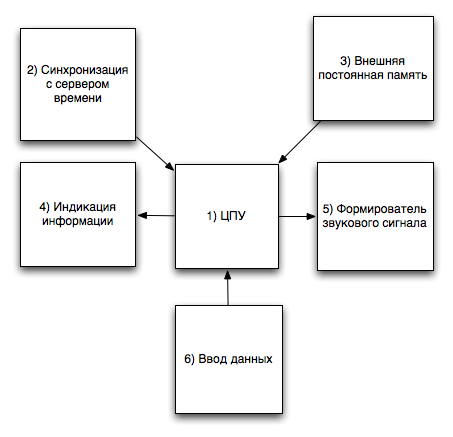
\includegraphics[bb=0 0 453 437, clip, scale=0.8]{funcd.png}}
% 	\caption{Фнкциональная структура}
% 	\label{img:funcd}
% \end{figure}
% 
% 
\subsection{Детализация компонентов универсальной системы терморегулирования}

\subsection{Анализ динамики работы системы}

\subsection{Разработка контроллирующего серсива}

\subsubsection{Описание методики обеспечения отказоустойчивости контроллирующего
сервиса}

\subsubsection{Описание протокола взаимодейства управляющего устройства с
контроллирующим сервисом}

\subsection{Разработка сервиса обслуживания запросов операторов системы}
\subsubsection{Описание методики оптимизации программы обслуживания операторов
системы}
\subsubsection{Виды доступных операций}

\subsection{Разработка микропрограммы управляющего устройства}

% (http://www.complexdoc.ru/lib/ГОСТ%20Р%208.585-2001)
\subsubsection{Способ расчёта показателей датчиков температур по
ГОСТ Р 208.585-2001}
В качестве температурных датчиков устанавливаемых внутри объекта управления используются
термопары. Принцип получения показания температуры термопар основан на
термоэлектрическом эффекте Зеебека. Когда концы проводника находятся при разных температурах,
между ними возникает разность потенциалов, пропорциональная разности температур.
Коэффициент пропорциональности называют коэффициентом термоэдс.

Способ получения показаний температуры устройством управления универальной
ситемы терморегулирования осован на табличном методе поиска значения.
Основной его недостаток -- необходимость выделения 300 байт памяти микроконтроллера под
таблицу соответствия температуры и текущего показания термоэдс.
Однако он обладает следующими преимуществами:
\begin{itemize}
	\item{} сложность алгоритма вычисления значения температуры линецна и максимально занимает
		900 тактов;
	\item{} таблица соответствия может одновременно кодировать значение термоэдс с поправкой на
		ошибку считанного значения термоэдс, что необходимо выполнять ввиду нелинейной зависимости
		температуры и термоэдс, разброса чувствительности термопар составляющей 10-15\%, ошибки
		вносимой операционным усилителем, ошибки вносимой способом монтажа термопары на печатной плате;
	\item{} отсутствует необходимость использовать прецизионные сопротивления делителя
		напряжения операционного усилителя.
\end{itemize}

Для получения текущего значения температуры используется следующая формула:
\begin{equation}
	T_i = min_{tbl}(Adc(E_i \times{} K_{amp}) > x) 
\end{equation}
\begin{ESKDexplanation}
	\item[где ]{} $K_{amp}$ -- коэффициент усиления операционного уилителя,
	\item{} $E_i$ -- значение термоэдс,
	\item{} $T_i$ -- значение температуры,
	\item{} $Adc()$ -- функция преобразования аналогово сигнала в цифровой.
\end{ESKDexplanation}


Например для термопары типа Т, текущей температуры $1^oC$, $K_{amp}$ равным 100 и опорным напряжением
АЦП микроконтроллера 3.3 В получим:
$E_i = 0.000043$ В. Разрешение АЦП $= \frac{3.3}{2^{12}} = 0.000805$ В. Один градус температуры
кодируется $\frac{E_i \times{} K_{amp}}{\frac{3.3}{2^{12}}} = 5.34 $ значениями
беззнакового пребразования АЦП, а измеряемый диапазон температур составит от $0^oC$ до $862^oC$,
что в 4 раза превышает необходимую разрешающую способность.


\subsubsection{Алгоритм управления силовой нагрузкой}

\subsubsection{Алгоритм сетевого взаимодействия управляющего устройства
с контоллирующим сервером}

\subsubsection{Методика применения AES шифрования данных передаваемых
контроллирующему сервису}

\subsubsection{Методика понижения потребляемого тока управляющим устройством
программным способом}

\subsubsection{Описание структуры классов микропрограммы управляющего устройства}
